\documentclass[a4paper]{article}
\usepackage{listings}
\usepackage{geometry}
\usepackage[parfill]{parskip}
\usepackage[bottom]{footmisc}

\usepackage[bookmarks=true, bookmarksopen=true]{hyperref}
\usepackage{bookmark}
\usepackage{enumitem}
\usepackage{color}
\definecolor{linkcolour}{rgb}{0,0.2,0.6}
\hypersetup{colorlinks, breaklinks, urlcolor=linkcolour, linkcolor=linkcolour}

\usepackage{amsmath, bm}
\newcommand{\norm}[1]{\left\lVert#1\right\rVert}

\usepackage{csvsimple}

% Font
\usepackage{fontspec}
\setmainfont{GFS Artemisia}

\renewcommand{\figureautorefname}{Σχήμα}
\renewcommand{\tableautorefname}{Πίνακας}

% Images
\usepackage{graphicx}
\graphicspath{{../figures/}}
\usepackage[font={footnotesize,it}]{caption}
\usepackage[font={footnotesize}]{subcaption}
\renewcommand{\thesubfigure}{\Roman{subfigure}}
\usepackage{float}

% English-Greek use
\usepackage{polyglossia}
\setmainlanguage{greek}
\setotherlanguage{english}

% References
\usepackage[backend=biber,style=alphabetic]{biblatex}
\addbibresource{references.bib}

\geometry{
 a4paper,
 total={170mm,257mm},
 left=20mm,
 top=20mm,
}

\title{Βαθιά Μάθηση και Ανάλυση Πολυμεσικών Δεδομένων \\ Τρίτη Εργασία}
\author{Κωστινούδης Ευάγγελος \\ΑΕΜ: 112}
\date{\today}

\begin{document}
\maketitle
\pagenumbering{gobble}
\newpage
\pagenumbering{arabic}

\section{Περιγραφή προβλήματος που επιλέχτηκε}

Για την εργασία αυτή επιλέχτηκε το πρόβλημα του Lunar Lander από την βιβλιοθήκη
του
\href{https://gymnasium.farama.org/environments/box2d/lunar_lander/}{Gymnasium}.
Το περιβάλλον αυτό έχει ως κατάσταση (state) ένα διάνυσμα 8 διαστάσεων και ως
κινήσεις (actions) είναι 4 και είναι διακριτές.

Οι αλγόριθμοι που επιλέχτηκαν για την επίλυση του προβλήματος είναι οι:

\begin{enumerate}
\item Deep Q-Learning (DQN)
\item Proximal Policy Optimization (PPO)
\end{enumerate}


\section{Deep Q-Learning}

Χρησιμοποιήθηκε ο αλγόριθμος του double deep Q-learning για την επίλυση του
προβλήματος. Το δίκτυο αποτελείται από δύο κρυφά επίπεδο με 64 νευρώνες. Η
συνάρτηση ενεργοποίησης που χρησιμοποιήθηκε είναι η relu. Στο επίπεδο εξόδου δεν
χρησιμοποιήθηκε καμία συνάρτηση ενεργοποίησης.

Το μέγεθος της μνήμης των προηγούμενων κινήσεων είναι $10.000$. Η πιθανότητα με
την οποία πραγματοποιείται μία τυχαία κίνηση έχει αρχική τιμή $0.9$ στην αρχή
της εκπαίδευσης και μειώνεται εκθετικά μέχρι να φτάσει την τελική της τιμή που
είναι $0.05$.

Ο αλγόριθμος του double deep Q-learning χρησιμοποιεί δύο ίδια νευρωνικά δίκτυα
για τον υπολογισμό του Q ούτως ώστε να μην γίνεται υπερεκτίμηση της τιμής του.
Το ένα δίκτυο εκπαιδεύεται μέσω του back propagation του σφάλματος και το άλλο
ανανεώνεται βάση των τιμών του που έχει το άλλο δίκτυο. Ο τρόπος ανανέωσης των
παραμέτρων είναι:

\begin{equation*}
    param_{target} = \tau * param_{policy} + (1-\tau) * param_{target}
\end{equation*}

Όπου $param$ είναι κάθε παράμετρος του δικτύου, $target$ είναι το "σταθερό"
δίκτυο και $policy$ είναι το δίκτυο που εκπαιδεύεται μέσω του back propagation.
Η τιμή του $\tau$ είναι $0.001$.

Η εκπαίδευση πραγματοποιήθηκε για μέγιστο αριθμό επεισοδίων $2.000$. Αν
αθροιστική ανταμοιβή (reward) του επεισοδίου είναι μεγαλύτερη του $250$, τότε η
εκπαίδευση σταματάει. Ο αλγόριθμος εκπαίδευσης είναι ο Adam με συντελεστή
μάθησης $0.001$

Στο παρακάτω διάγραμμα παρουσιάζεται η καμπύλη των αθροιστικών ανταμοιβών
(rewards) και πιθανότητας επιλογής τυχαίων κινήσεων για κάθε επεισόδιο.
Παρατηρούμε ότι η εκπαίδευση σταμάτησε στο 180 επεισόδιο επειδή το reward
ξεπέρασε την τιμή του 250.

\begin{figure}[H]
    \centering

    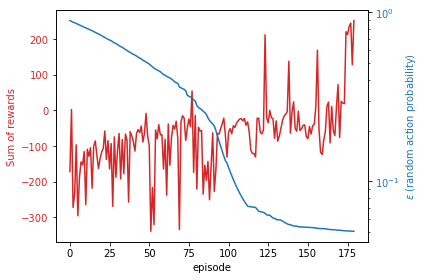
\includegraphics[width=.8\linewidth]{dqn_reward_epsilon.png}

    \caption{Διάγραμμα αθροιστικών ανταμοιβών (rewards) και πιθανότητας επιλογής
    τυχαίων κινήσεων για κάθε επεισόδιο.}
\end{figure}


\section{Proximal Policy Optimization}

Ο PPO είναι ένας αλγόριθμος actor critic. Η αρχιτεκτονική των νευρωνικών δικτύων
που χρησιμοποιήθηκε αποτελείται από δύο κρυφά επίπεδα με 64 νευρώνες το καθένα.
Η συνάρτηση ενεργοποίησης που χρησιμοποιήθηκε είναι η υπερβολική εφαπτομένη. Η
διαφορά τους είναι ότι ο actor έχει ένα επίπεδο softmax στην έξοδο, ενώ ο critic
δεν έχει τίποτα.

Σε κάθε επεισόδιο πραγματοποιούνται 16 παράλληλες προσομοιώσεις όπου κάθε
προσομοίωση διαρκεί 1024 κινήσεις. Αν μία προσομοίωση τερματίζεται, τότε
επανέρχεται στην αρχική της κατάσταση και επαναλαμβάνεται η προσομοίωση.

Για την εκπαίδευση των δικτύων σε κάθε επεισόδιο χρησιμοποιούνται 5 εποχές και ο
αριθμός των batches είναι 32. Οι σταθερές της συνάρτησης κόστους είναι $0.5$ για
το σφάλμα του critic και $0.01$ για της εντροπία. Η τιμή του clip είναι $0.2$.
Τέλος, η εκπαίδευση έγινε για 200 επεισόδια.

Στο παρακάτω διάγραμμα παρουσιάζονται το μέσο των αθροιστικών ανταμοιβών για
κάθε προσομοίωση (τόσο για όσες έχουν τελειώσει, όσο και γι᾽ αυτές που δεν
τελείωσαν) και ο αριθμός των προσομοιώσεων που τερμάτισαν για κάθε επεισόδιο.

\begin{figure}[H]
    \centering

    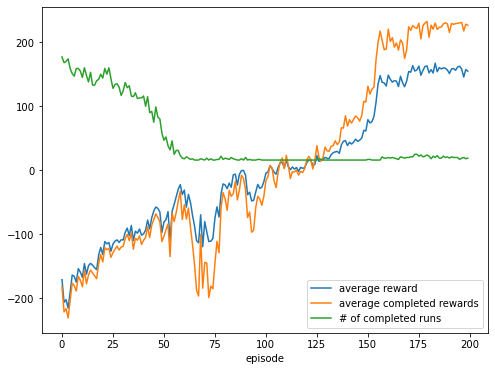
\includegraphics[width=.8\linewidth]{ppo_rewards.png}

    \caption{Το μέσο των αθροιστικών ανταμοιβών για κάθε προσομοίωση (τόσο για
    όσες έχουν τελειώσει, όσο και γι᾽ αυτές που δεν τελείωσαν) και ο αριθμός των
    προσομοιώσεων που τερμάτισαν για κάθε επεισόδιο.}
\end{figure}

Στο παρακάτω διάγραμμα παρουσιάζονται τα σφάλματα για κάθε επεισόδιο.

\begin{figure}[H]
    \centering

    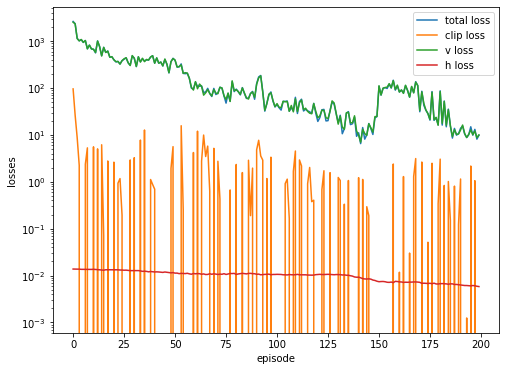
\includegraphics[width=.8\linewidth]{ppo_losses.png}

    \caption{Διάγραμμα σφαλμάτων για κάθε επεισόδιο.}
\end{figure}


\end{document}
